\documentclass{standalone}
\usepackage{tikz}
\usetikzlibrary{bbox, angles, quotes}
\usetikzlibrary{calc}
\usetikzlibrary{arrows.meta,decorations.pathmorphing,backgrounds,positioning,fit,petri}

\def\b{0.05}
\def\centerarc[#1](#2)(#3:#4:#5)% Syntax: [draw options] (center) (initial angle:final angle:radius)
    { \draw[#1] ($(#2)+({(#5)*cos(#3)},{(#5)*sin(#3)})$) arc (#3:#4:#5); }

\def\beamline[#1](#2)(#3:#4)% Syntax: [draw options] (radius) (initial angle:final angle:radius)
    {  \draw[#1] ({(#2-2*\b)*cos(#4)},-#3/2 * sin(#4)) -- ({(#2-2*\b)*cos(#4)},#3/2 * sin(#4)); 
    \draw ({(1-2*0.05)*cos(90)},{-1/2 * sin(90)}) -- ({(1-2*0.05)*cos(90)},{1/2 * sin(90)});
    }


\begin{document}

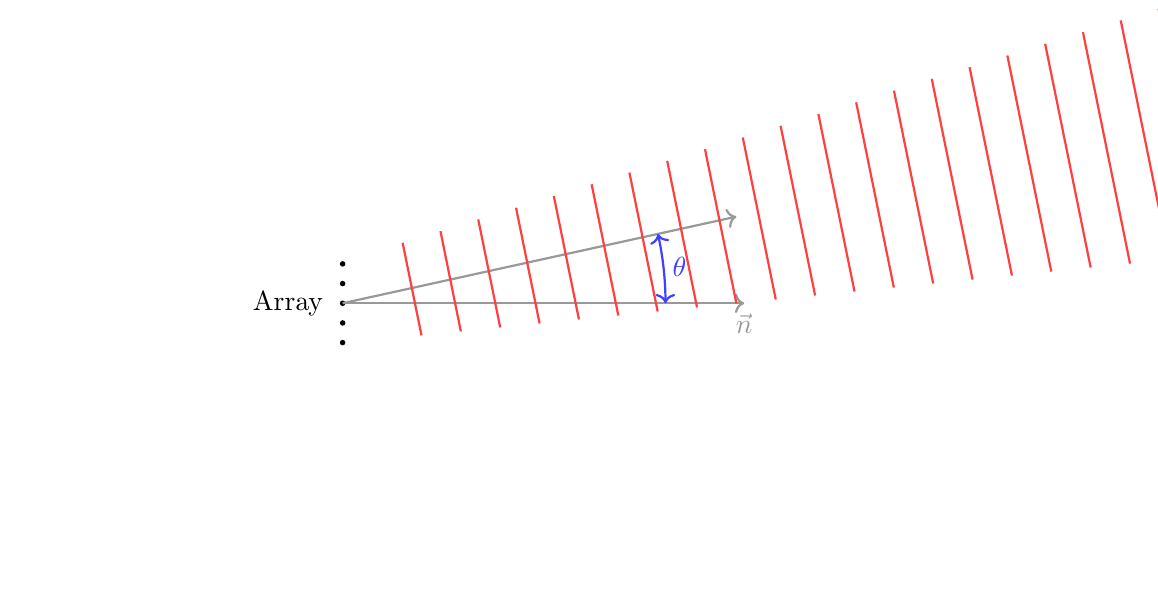
\begin{tikzpicture}
    [wave/.style={white!80!black,thin},
    wave1/.style={white!25!red,thick},
    angle1/.style={white!25!blue,thick},
    wave2/.style={white!60!black,thick}]
%    \coordinate[label={S}] (origin) at (0,2.5);
%   \fill[red] (origin) circle (2pt);

%   \centerarc[wave](origin)(0:360:0.5)
%    \centerarc[wave](origin)(0:360:1)
%    \centerarc[wave](origin)(0:360:1.5)
%    \centerarc[wave](origin)(0:360:2.0)
%    \centerarc[wave](origin)(0:360:2.5)
%    \centerarc[wave](origin)(0:360:3)
%    \centerarc[wave](origin)(0:360:3.5)
%    \centerarc[wave](origin)(0:360:4)
%    \centerarc[wave](origin)(0:360:4.5)
%    \centerarc[wave](origin)(0:360:5.0)
%    \centerarc[wave](origin)(0:360:5.5)

    \coordinate[] (m1) at (0, -0.5);
    \coordinate[] (m2) at (0, -2/8);
    \coordinate[] (m21) at (0, -3/8);
    \coordinate[] (m22) at (0, -1/8);
    \coordinate[] (m3) at (-0.0,0);
    \coordinate[] (m4) at (0, 2/8);
    \coordinate[] (m5) at (0, 0.5);
    \coordinate[] (n1) at (5.1, 0);
    \coordinate[] (d1) at (5, 1.1);
    \fill (m1) circle (1pt);
    \fill (m2) circle (1pt);
    \fill (m3) circle (1pt);
    \fill (m4) circle (1pt);
    \fill (m5) circle (1pt);

    \draw [->, wave2] (m3) -- (n1) node[right,below]{$\vec{n}$};
    \draw [->, wave2] (m3) -- (d1) ;
    
    \foreach \i in {0,...,20}
    {
        \centerarc[wave](m1)(0:360:1 + \i*0.5)    
    }
    \foreach \i in {0,...,20}
    {
        \centerarc[wave](m2)(0:360:-1*\b + 1 + \i*0.5)    
    }
    \foreach \i in {0,...,20}
    {
        \centerarc[wave](m3)(0:360:-2*\b + 1 + \i*0.5)    
    }
    \foreach \i in {0,...,20}
    {
        \centerarc[wave](m4)(0:360:-3*\b + 1 + \i*0.5)    
    }
    \foreach \i in {0,...,20}
    {
        \centerarc[wave](m5)(0:360:-4*\b + 1 + \i*0.5)    
    }

%    \draw (1-2*\b,1) -- (1-2*\b,-1);
%    \beamline[wave](1)(1:1)
    \node[label=left:{Array}] at (-0.0,0) {};
    \begin{scope}[transform canvas={rotate=11.5}]
        \foreach \i in {0,...,20}
        {
            \draw[wave1] (\i * 0.5 + 1-2*\b, -0.6-0.05*\i) -- (\i * 0.5 + 1-2*\b, 0.6 + 0.05*\i);
        }
    \end{scope}
    \pic [draw, <->, angle1,
    angle radius=41mm, angle eccentricity=1.05,"$\theta$"] {angle = n1--m3--d1};
    \pgfresetboundingbox
%    \useasboundingbox(-2.6,-2.6)rectangle(2.6,3.6);
    \useasboundingbox(-4,-3.5)rectangle(10,3.5);
\end{tikzpicture}
\end{document}